\documentclass{article}\usepackage[]{graphicx}\usepackage[]{color}
% maxwidth is the original width if it is less than linewidth
% otherwise use linewidth (to make sure the graphics do not exceed the margin)
\makeatletter
\def\maxwidth{ %
  \ifdim\Gin@nat@width>\linewidth
    \linewidth
  \else
    \Gin@nat@width
  \fi
}
\makeatother

\definecolor{fgcolor}{rgb}{0.345, 0.345, 0.345}
\newcommand{\hlnum}[1]{\textcolor[rgb]{0.686,0.059,0.569}{#1}}%
\newcommand{\hlstr}[1]{\textcolor[rgb]{0.192,0.494,0.8}{#1}}%
\newcommand{\hlcom}[1]{\textcolor[rgb]{0.678,0.584,0.686}{\textit{#1}}}%
\newcommand{\hlopt}[1]{\textcolor[rgb]{0,0,0}{#1}}%
\newcommand{\hlstd}[1]{\textcolor[rgb]{0.345,0.345,0.345}{#1}}%
\newcommand{\hlkwa}[1]{\textcolor[rgb]{0.161,0.373,0.58}{\textbf{#1}}}%
\newcommand{\hlkwb}[1]{\textcolor[rgb]{0.69,0.353,0.396}{#1}}%
\newcommand{\hlkwc}[1]{\textcolor[rgb]{0.333,0.667,0.333}{#1}}%
\newcommand{\hlkwd}[1]{\textcolor[rgb]{0.737,0.353,0.396}{\textbf{#1}}}%
\let\hlipl\hlkwb

\usepackage{framed}
\makeatletter
\newenvironment{kframe}{%
 \def\at@end@of@kframe{}%
 \ifinner\ifhmode%
  \def\at@end@of@kframe{\end{minipage}}%
  \begin{minipage}{\columnwidth}%
 \fi\fi%
 \def\FrameCommand##1{\hskip\@totalleftmargin \hskip-\fboxsep
 \colorbox{shadecolor}{##1}\hskip-\fboxsep
     % There is no \\@totalrightmargin, so:
     \hskip-\linewidth \hskip-\@totalleftmargin \hskip\columnwidth}%
 \MakeFramed {\advance\hsize-\width
   \@totalleftmargin\z@ \linewidth\hsize
   \@setminipage}}%
 {\par\unskip\endMakeFramed%
 \at@end@of@kframe}
\makeatother

\definecolor{shadecolor}{rgb}{.97, .97, .97}
\definecolor{messagecolor}{rgb}{0, 0, 0}
\definecolor{warningcolor}{rgb}{1, 0, 1}
\definecolor{errorcolor}{rgb}{1, 0, 0}
\newenvironment{knitrout}{}{} % an empty environment to be redefined in TeX

\usepackage{alltt}
\usepackage[hmargin = 1in]{geometry}
\usepackage{enumitem}
\usepackage{amsmath, amsthm, amssymb, amsfonts}
\setlist[2]{
font = \color{black},
before = {\color{red}}
}
\usepackage{textcomp}
\IfFileExists{upquote.sty}{\usepackage{upquote}}{}
\begin{document}









\begin{center} \LARGE
Homework 13
\end{center}
\begin{center} \Large
Due April 30, 2020 at 11:59 PM 
\end{center}



\begin{enumerate}
	\item P. 533: 1 (ignore (f), (g)) (14 points for (d), 6 points for others), dataset: {\tt pencil.jmp} 
	\begin{itemize}
	\item[(a)]
	Data within each sample must be iid normal, the samples must be independent, and the three distributions must have the same standard deviation.
\begin{knitrout}
\definecolor{shadecolor}{rgb}{0.969, 0.969, 0.969}\color{fgcolor}

{\centering 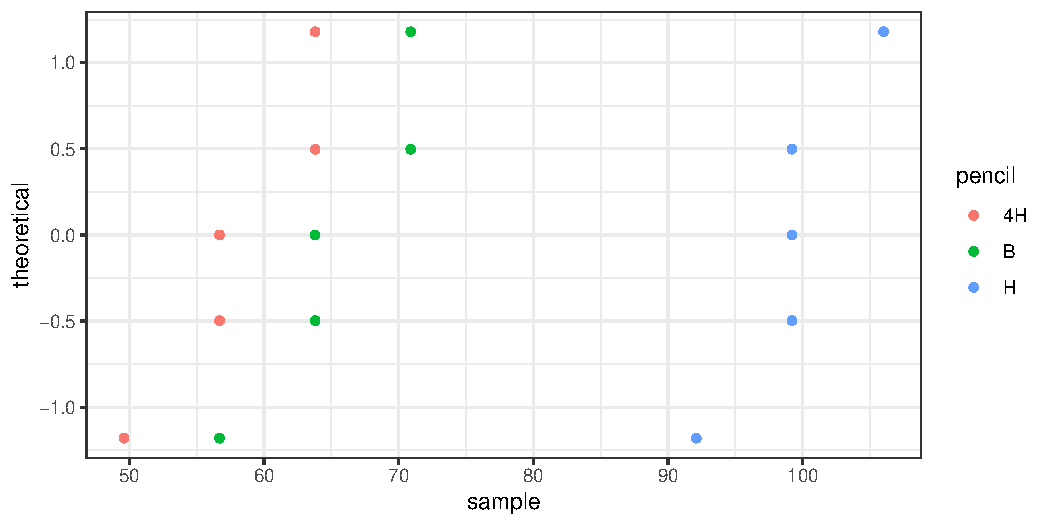
\includegraphics[width=0.7\textwidth]{figure/unnamed-chunk-2-1} 

}



\end{knitrout}
\begin{knitrout}
\definecolor{shadecolor}{rgb}{0.969, 0.969, 0.969}\color{fgcolor}

{\centering 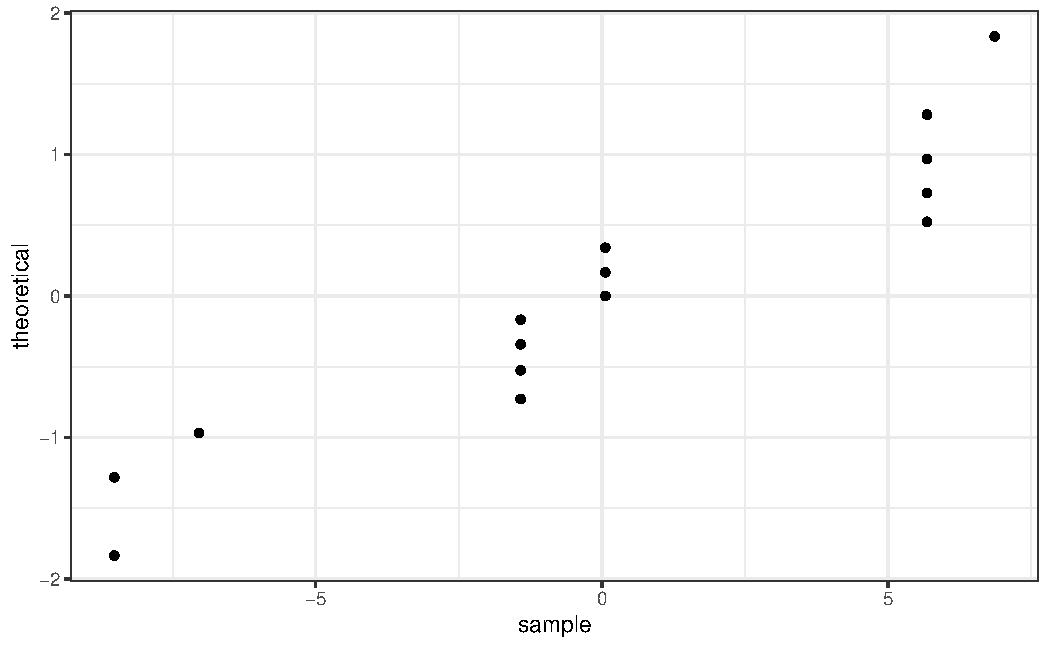
\includegraphics[width=0.6\textwidth]{figure/unnamed-chunk-3-1} 

}



\end{knitrout}
  
  The three normal plots of the data are roughly linear with no outliers, providing no evidence against the normal part of the assumption. The slopes are also similar, providing no evidence against the common standard deviation assumption. The normal plot of the residuals is roughly linear (considering the number of ties). This also provides nor evidence against the normal part of the assumption.
  
  \item[(b)]
  Using equation (7.7) in the textbook, $s_P^2 = 31.57733$, and so $s_P = \sqrt{31.57733} = 5.619$, with $n - r = 15 - 3 = 12$ degrees of freedom associated with it. This measures the magnitude of baseline variation within any of the 3 conditions, assuming it is the same for all 3 conditions.
  
  \item[(c)]
  Use equation (7.14). The $\pm$ part (margin of error) is the same for all three intervals because all three sample size are the same. For 95\% confidence, the quantile used is $t_{n - r, 1 - \alpha/2} = t_{12, 0.975} = 2.179$. So the margin of error is
  \[t_{12, 0.975} s_P \sqrt{\frac{1}{n_i}} = 2.179 \frac{5.619}{\sqrt{5}} = 5.475956\]
  The confidence intervals are 
  \[\hat{\mu}_i \pm t_{12, 0.975} s_P \sqrt{\frac{1}{n_i}}, i = 4H, H, B\]
  Plugging in $\hat{\mu}_i$ in the JMP output and the margin of error, we have the confidence intervals for $\mu_{4H}, \mu_{H}, \mu_{B}$ are  
  \[(52.64, 63.60), (93.66, 104.62), (59.74, 70.70)\]
  respectively.
  
  \item[(d)]
  Use equation (7.15). The margin of error is the same for all 3 intervals because all three sample sizes are the same. The quantile used is the same as in (c). The margin of error is
  \[t_{12, 0.975} s_P \sqrt{\frac{1}{n_i} + \frac{1}{n_j}} = 2.179 (5.619)\sqrt{\frac{1}{5} + \frac{1}{5}}\]
  Using the $\hat{\mu}_i$ in the JMP output, the resulting confidence intervals for $\mu_{4H} - \mu_{H},\, \mu_{4H} - \mu_{B},\, \mu_{H} - \mu_{B}$ are 
  \[(-48.76, -33.28), (-14.83, 0.64), (26.18, 41.66)\]
  respectively.
  
  \item[(e)]
  Label the 4H lead Sample 1, the H lead Sample 2 and the B lead Sample 3. Use equation (7.20) with $c_1 = c_2 = 1/2,\, c_3 = -1$. The quantile used is the same $t_{12. 0.975}$ as in (c). The resulting interval is
  \begin{align*}
  &\frac{\hat{\mu}_1 + \hat{\mu}_2}{2} - \hat{\mu}_3 \pm t_{12, 0.975} s_P \sqrt{\frac{(1/2)^2}{n_1} + \frac{(1/2)^2}{n_2} + \frac{(-1)^2}{n_3}}\\
  =& \frac{58.12 + 99.14}{2} - 65.2213 \pm 2.179 (5.619) \sqrt{\frac{1/4 + 1/4 + 1}{5}}\\
  =& 13.41 \pm 6.706649\\
  =& (6.70, 20.12)
  \end{align*}
  
  \item[(h)]
  \begin{enumerate}[label = \arabic*.]
  \item $H_0: \mu_1 = \mu_2 = \mu_3,\, H_a: $ not all $\mu_1, \mu_2, \mu_3$ are the same
  \item
  The test statistic is 
  \[F = \frac{SSR/(r - 1)}{SSE/(n - r)}.\]
  Assuming $H_0$ is true and the model $Y_{ij} = \mu_i + \epsilon_{ij},\, \epsilon_{ij} \sim N(0, \sigma^2)$ is valid. The test statistic $F \sim F_{2, 12}$. 
  \item The observed $F$ in the JMP output is 76.10. The p-value is
  \[P(F_{2,12} > 76.10) < 0.0001\]
  \item
  The p-value is small, so we reject $H_0$ and conclude $H_a$.
  \item
  There is overwhelming evidence that all 3 leads do not produce the same mean strength.
  \end{enumerate}
  \item[(i)]
  The ANOVA table is given below.
  \begin{center}
  \begin{tabular}{lrrrr}
  \hline
  Source & SS & df & MS & F\\ \hline
  Treatment & 4806.0 & 2 & 2403.0 & 76.10\\
  Error & 378.9 & 12 & 31.6 & \\ \hline
  Total & 5185.0 & 14 &&\\ \hline
  \end{tabular}
  \end{center}
	\end{itemize}
	
\end{enumerate}
%\newpage 
%\nocite{*}
%\bibliographystyle{plainnat} 
%\bibliography{}
\end{document}
